\section{Data and preprocessing}
\section{Data description}
One of the most straightforward way to deal with the limit amount of available data is to leverage as much related Medical Data as possible. We thus investigated several public available dataset for Lung CT scans in addition to the Covid-CT dataset.

\subsection{NSCLC Dataset}
NSCLC Dataset contains 402 Lung CT scans, of which 78 cases are anotated with left lung, right lung and pleural effusion area. A sample annotation is shown in figure \ref{fig:NSCLC_example}
\begin{figure}[h]
	\centering
	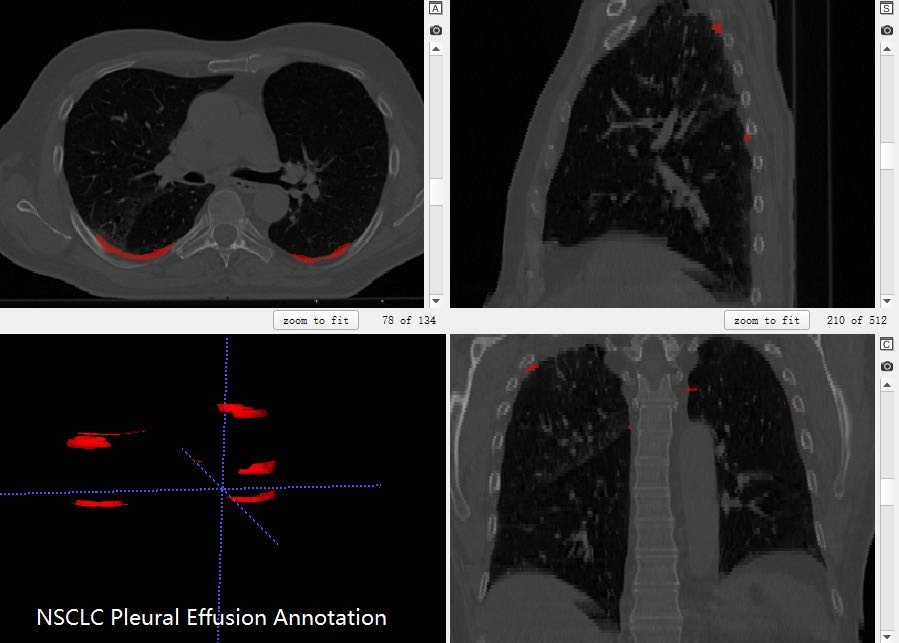
\includegraphics[width=0.6\textwidth]{img/Dataset/NSCLC}
	\caption{An example volume from NSCLC Dataset with its annotation}
	\label{fig:NSCLC_example}
\end{figure}

\subsection{MSD Lung Tumor}
MSD Lung Tumor contains 63 Lung CT scans, annotating the Lung Cancer area. An example shown in figure \ref{fig:MSD_example}
\begin{figure}[h]
	\centering
	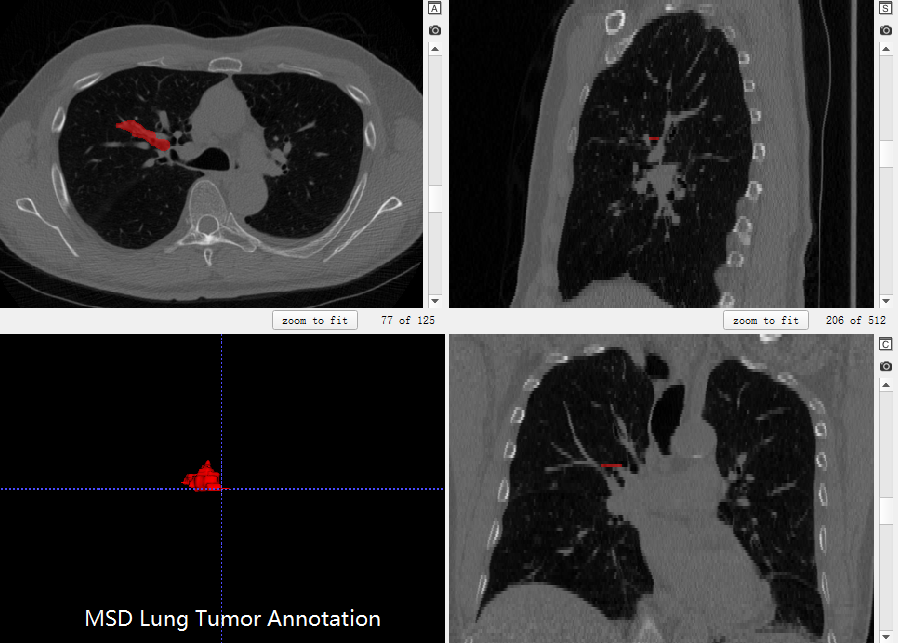
\includegraphics[width=0.6\textwidth]{img/Dataset/MSD}
	\caption{An example volume from MSD Dataset with its annotation}
	\label{fig:MSD_example}
\end{figure}

\subsection{MosMed Dataset}
MosMed Dataset Contains 50 Annotated thick-slice Covid CT scans, as well as around 300 unannotated Lung CTs. We'd like to report here that we used only 200 unannotated slices because downloading keep giving me error due to location restriction. An example shown in figure \ref{fig:MosMed_example}
\begin{figure}[h]
	\centering
	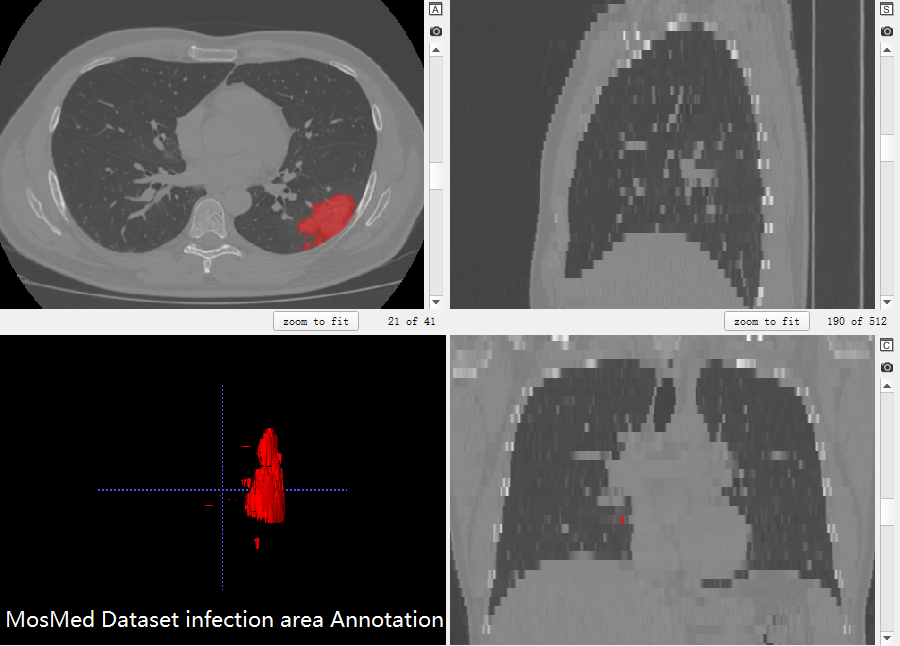
\includegraphics[width=0.6\textwidth]{img/Dataset/MosMed_example}
	\caption{An example volume from MosMed Dataset with its annotation}
	\label{fig:MosMed_example}
\end{figure}


\subsection{Covid Segmentation Benchmark}
Covid Segmentation Benchmard contains 20 CT scans from 2 radiometric centers, of which 10 volumes thin-slice CT volumes and 10 thick slice CT volumes.
\begin{figure}[h]
	\centering
	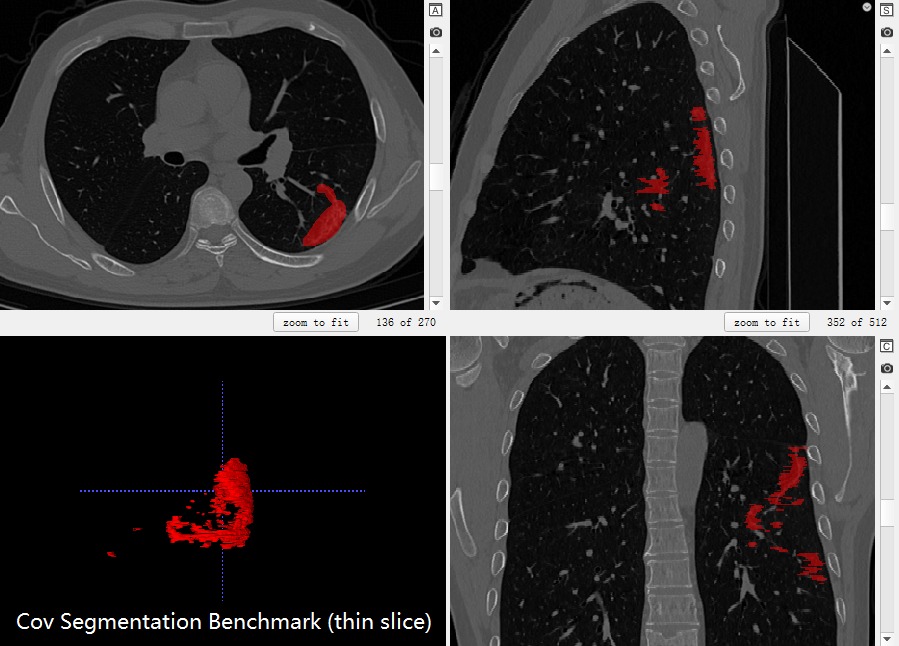
\includegraphics[width=0.6\textwidth]{img/Dataset/Cov_benchmark_thin}
	\caption{An example volume from Cov Segmentation Benchmark (thin slice) with its annotation}
	\label{fig:Covseg_thin}
\end{figure}
\begin{figure}[h]
	\centering
	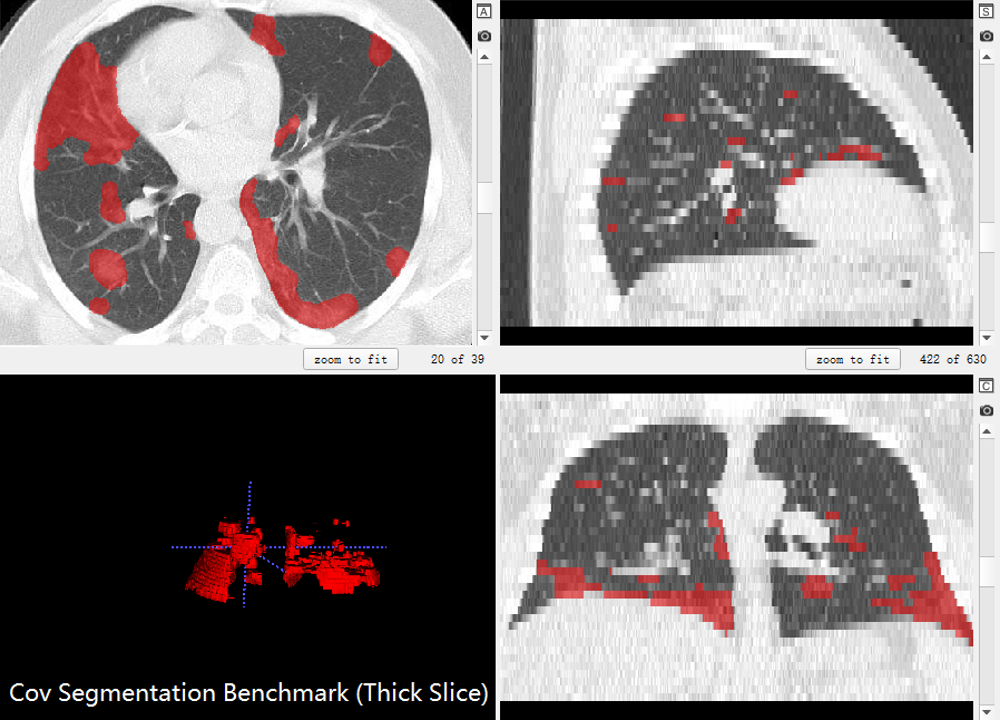
\includegraphics[width=0.6\textwidth]{img/Dataset/Cov_benchmark_thick}
	\caption{An example volume from Cov Segmentation Benchmark (thick slice) with its annotation}
	\label{fig:Covseg_thick}
\end{figure}


\section{Data preprocessing}
The dataset used in this paper was collected from multiple centers with different equipment setup. Structseg2019, NSCLC, MSD Lung Tumor set are thin slice CT scans. MosMed contained 50 thick slice scans and the Covid segmentation benchmark are multi-center dataset from different centers. We argue that deep learning algorithms, especially segmentation tasks are sensitive to this difference. To make most use of the data, we first extract the lungs from the CT volumes. Then a sequence of preprocessing was performed including resampling, histogram equalization, and mean variance normalization. Most implementation used SimpleITK dataset

\subsection{Processing into functional features}
Lung CT scans images includes the lung tissue as well as bones and meshes that influence the preprocessing such as normalization as well as future segmentation. We intended to first segment the lung tissue out for better focus.\\
\textbf{Lung segmentation using watershed algorithm}\\

\textbf{Lung segmentation Using pre-trained Deep learning models}\\
Deep learning method provide finer results when facing severe pathology. Work in \cite{hofmanninger_automatic_2020} provided a promising result for Lung segmentation. In addition, they further improve their lung segmentation model with Covid-19 Lung data.\\

We leveraged their models provided in their github repository \footnote{https://github.com/JoHof/lungmask}. Original volumes from the Lung datasets went through the model, we threshold the lung out and set the uninterested area (background) as 0. Figure \ref{fig:filtered_Lung} showed and example lung volume before and after filtering the lung tissue.

\begin{figure}[h]
\centering
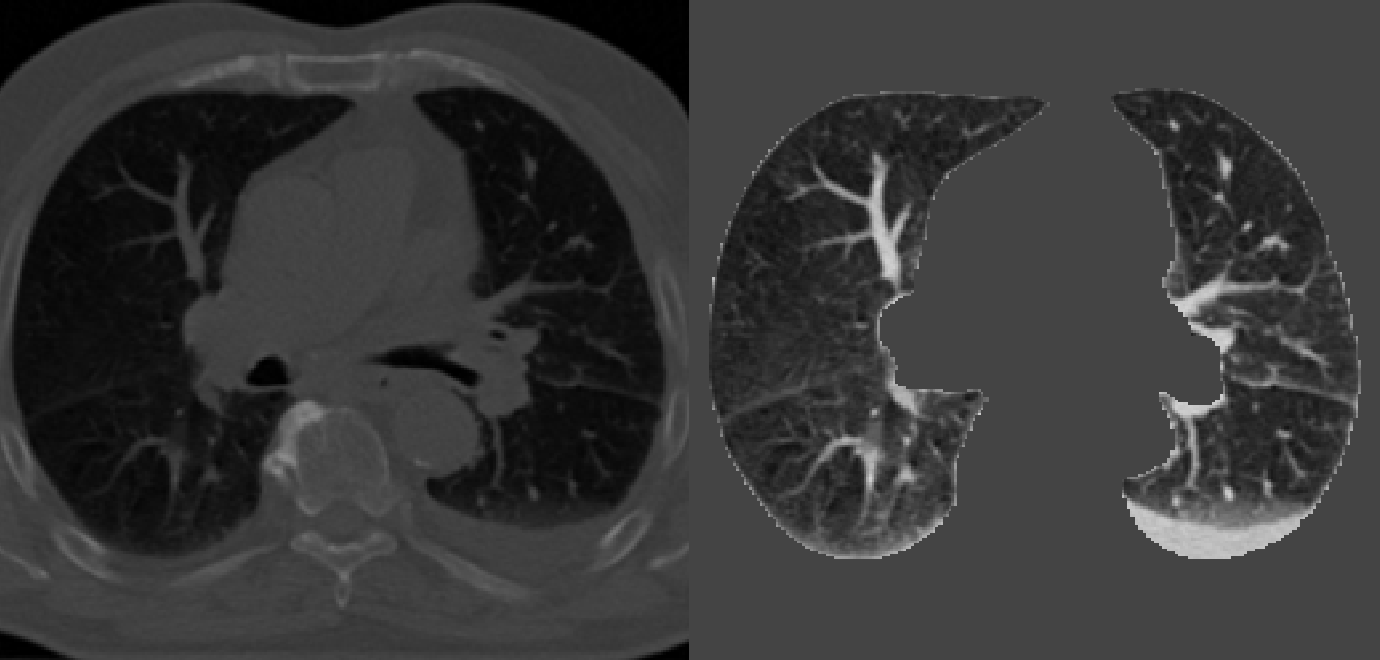
\includegraphics[width=0.5\textwidth]{/Users/tianyangsun/Desktop/Project/MSc-report/img/filtered_lung/nsclc_filteredlung_axial.png}
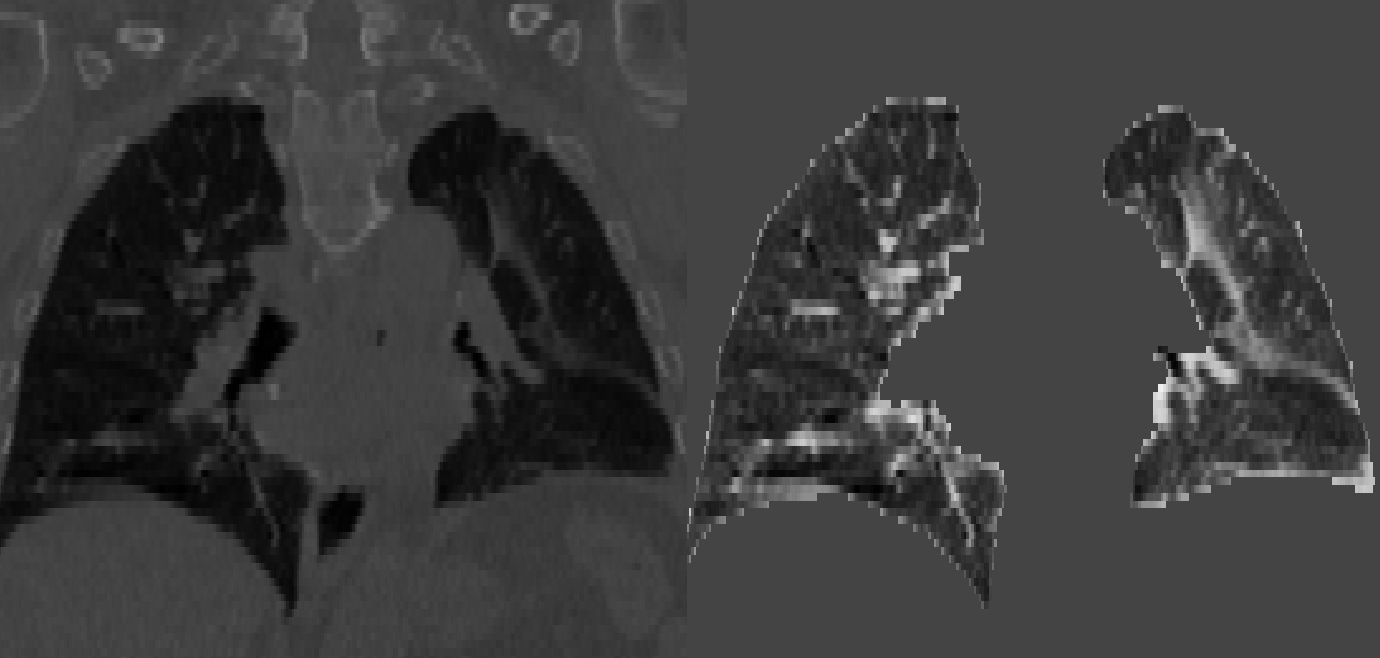
\includegraphics[width=0.5\textwidth]{img/filtered_lung/nsclc_filtered_coronal.png}
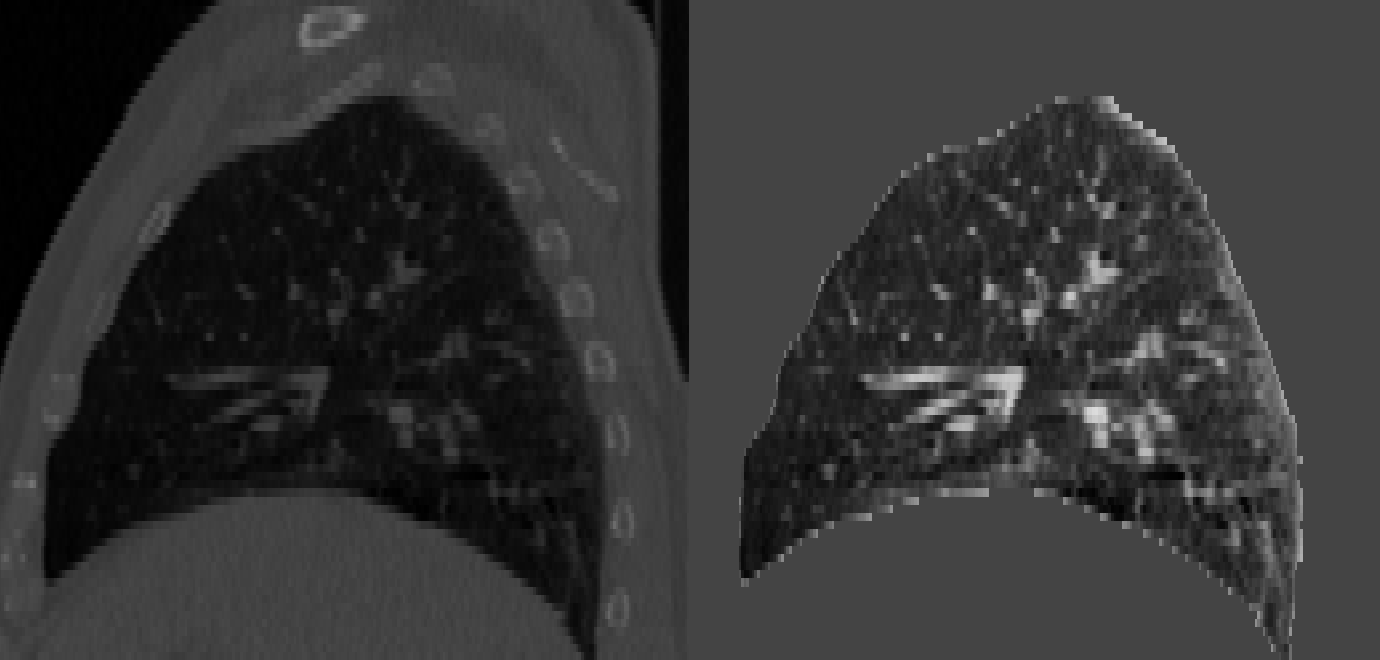
\includegraphics[width=0.5\textwidth]{/Users/tianyangsun/Desktop/Project/MSc-report/img/filtered_lung/nsclc_filteredlung_Saggital.png}
\caption{An example from NSCLC Pleural Effusion dataset showing the volumes before and after lung filtering. (Top: Axial view, Middle: Coronal view, Bottom: Saggital View)}
\label{fig:filtered_Lung}
\end{figure}

\subsection{Resampling}
\begin{figure}[h]
	\centering
	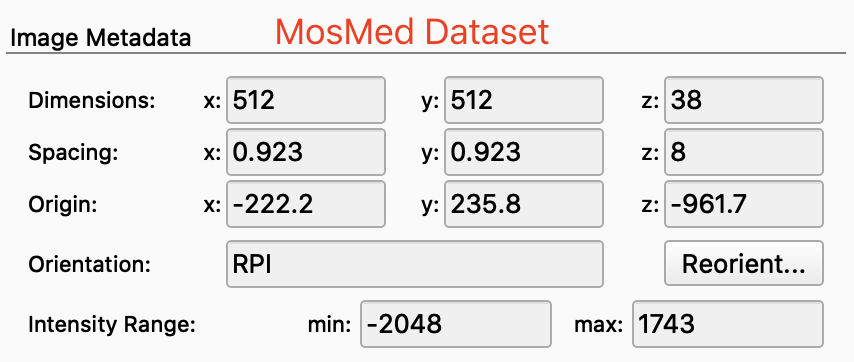
\includegraphics[width=0.5\textwidth]{/Users/tianyangsun/Desktop/Project/MSc-report/img/spacing_diverse/Mosmed_dataset.png}
	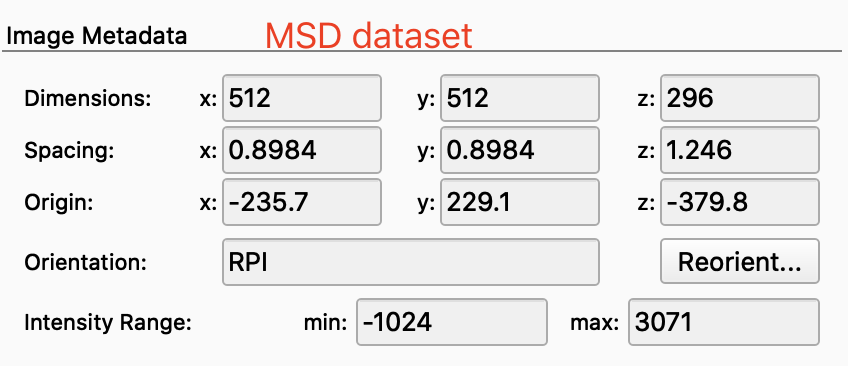
\includegraphics[width=0.5\textwidth]{/Users/tianyangsun/Desktop/Project/MSc-report/img/spacing_diverse/MSD_metadata.png}
	\caption{An example of different spacing information from MosMed and MSD dataset}
	\label{fig:Spacediverse}
\end{figure}
Figure \ref{fig:Spacediverse} showed the diveristy in spacing from different datsets. To deal with the different spacing for multi-domain data, we resampled the data to spacing (1, 1) in the Axial view and remain not changed in the Z axis.

\subsection{Mean Variance Normalization}
We performed Mean Variance Normalization (Z score normalization) for the lung tissue voxels by subtracting each volume with its mean and divided by its standard deviation. So that the data has zero mean and standard deviation of 1. 
$$z=\frac{x-\mu}{\sigma}$$ of which $\mu$ is the mean and $\sigma$ is the variance. Figure \ref{fig:normalization} showed the intensity range before and after normalization

\begin{figure}[h]
	\centering
	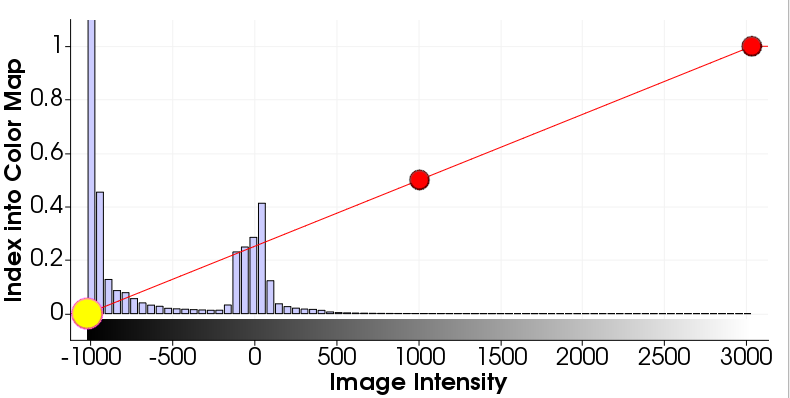
\includegraphics[width=0.5\textwidth]{/Users/tianyangsun/Desktop/Project/MSc-report/img/normalization/intensity_before.png}
	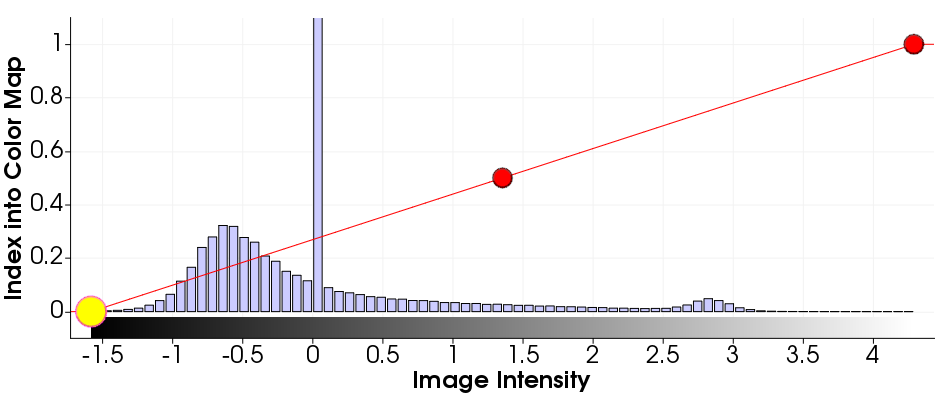
\includegraphics[width=0.5\textwidth]{/Users/tianyangsun/Desktop/Project/MSc-report/img/normalization/intensity_after.png}
	\caption{An example showing the intensity range before and after normalization (Top: before normalization; Bottom: after normalization)}
	\label{fig:normalization}
\end{figure}

\begin{figure}[h]
	\centering
	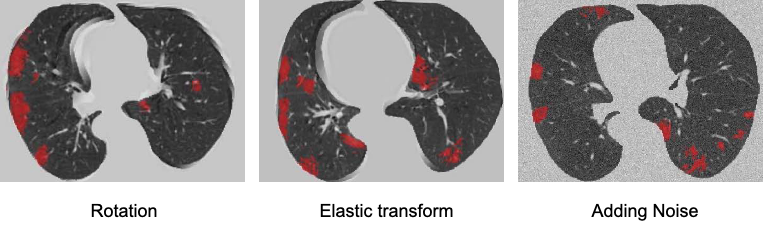
\includegraphics[width=\textwidth]{img/augment/rot_el_noise}
	\caption{Augmenting the data}
\end{figure}
\section{Data Augmentation}
% TODO: add examples showing the transformation in augmentation
For data augmentation, we investigated some of the augmentation techniques in medical imaging domain, each of the augmentation techniques was carefully chosen matching real medical situation.\\

\textbf{Rotation:} We performed a small random rotation between [-3, 3] degree considering the pose variation when lying down on the scanner.\\
%\begin{figure}[h]
%	\centering
%	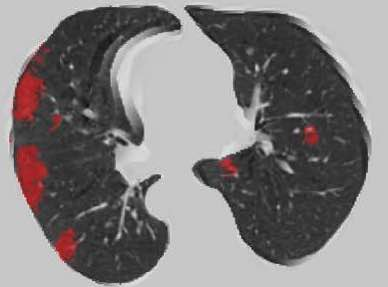
\includegraphics[width=0.4\textwidth]{img/augment/rotation}
%	\caption{An example of rotation using MosMed Dataset}
%\end{figure}

\textbf{Elastic Transformation:} We performed a small elastic transformation considering lying down and holding breath when scanning Lung CT might brings shape change to the lungs tissue.\\
%\begin{figure}[h]
%	\centering
%	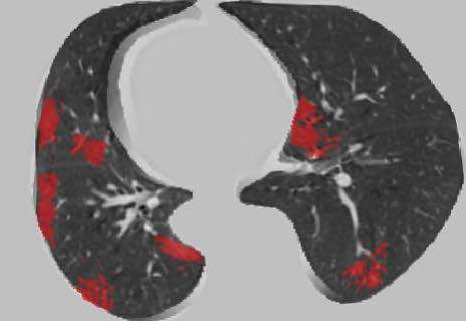
\includegraphics[width=0.4\textwidth]{img/augment/elastic_transformation}
%	\caption{An example of elastic transformation using MosMed Dataset}
%\end{figure}

\textbf{Random Gamma and Gaussian Noise:} We performed a random gamma correction to simulate the variation generate due to different equipment. We also added a random gaussian noise for a more robust training.

%\begin{figure}[h]
%	\centering
%	\includegraphics[width=0.4\textwidth]{img/augment/add_noise}
%	\caption{An example of random Gamma and Gaussian Noise using MosMed Dataset}
%\end{figure}





\newpage
\section{Experiment}
A good model, especially facing with small sample segmentation, should generalize well instead of overfitting on a small number of training data. The whole point of data augmentation, adding noise, etc, is to improve the generalizability of the trained neural network so that for the unseen data, the model predict reasonably well.\\

Due to the limited ability of the GPU resource available, tuning hyper-parameters using grid search is too inefficient. Thus in our experiment, we leveraged the optimizer scheduler in PyTorch so that starting from the learning rate starts from $lr=2\times10^{-4}$ and decreased to 0.8 * lr every 25 epochs so that the learning rate approach 0 in the later training stage.  
\begin{enumerate}
 	\item \textbf{Optimizer:} We used Adam optimizer considering that Model Genesis, winning solution for NSCLC segmentation as well as other well known solutions used the model optimizer.
	\item \textbf{Epochs:} The maximum number of epochs for training is 500. However, each epoch we validate the result and the best model was saved throughout the training process. We count the number of continued non-improving epochs, and when it reached 30 epochs, the training progress terminated automatically.
	\end{enumerate}

\section{With Fully labelled data}
We first consider training on a small dataset and all of them are labelled with segmentation masks, because this is the case during the first few months of this project when only 20 volumes of the Covid lungs from the Covid Segmentation benchmark were publicly available, later in July 2020, MosMed published a new dataset containing 50 labeled slices.

\subsection{Experiment Setup}
To fully leverage the Covid Dataset, we combined the 20 volumes in Covid Segmentation bechmark and the 50 volumes MosMed Dataset. We randomly selected 20 volumes for testing, and further split the 50 remaining volume into 5 fold for cross validation. Smaller sample: One fold (10 volumes) for training; Normal training: Four fold (40 Volumes) for training.
Note that since we cannot do anything to the various slice thickness, we sliced the volume into 2D.

\subsection{Best results}
For the segmentation of infection area using \textbf{fully labelled sample only}, we achieved Dice score (DSC) (40 volumes sliced in 2D for training and 10 for validation) 81.04\% on the validation set and 80.45\% on the testing set. All the volumes was preprocessed as described in Section 3 and augmented the data using random rotating, and elastic transformation on the training set only that generate augmentation no more than 50 percent of the training set.\\

For the segmentation of the infection area with the help of \textbf{unannotated samples}, our mean-teacher style training reported a small improvement and the teacher model is slightly out performed the student model that report 83.67\% on validation and 82.54 \% on the testing set.


\begin{figure}[h]
	\centering
	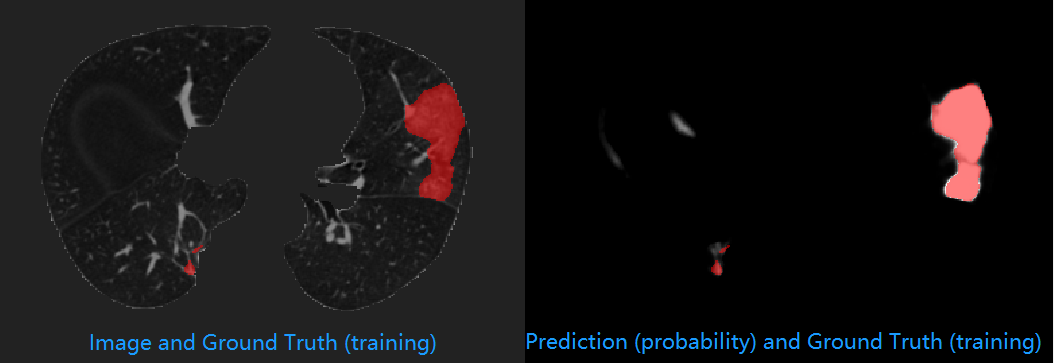
\includegraphics[width=0.8\textwidth]{img/experiment/Lung_result_train}
	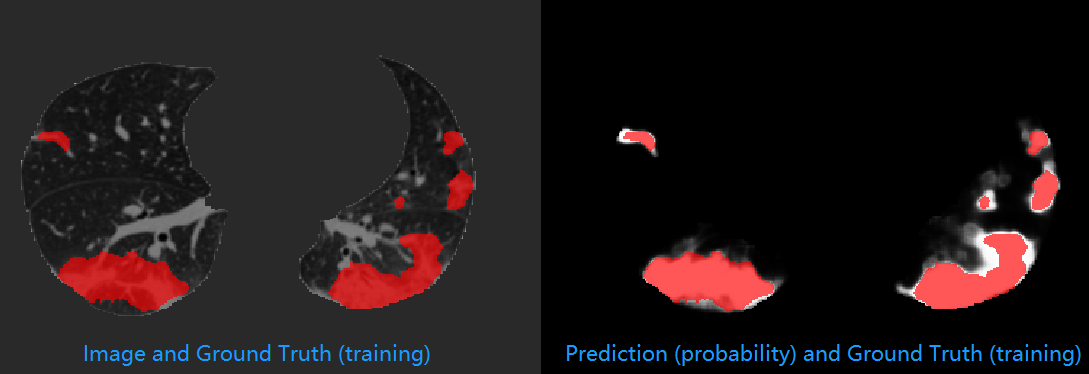
\includegraphics[width=0.8\textwidth]{img/experiment/Lung_result_train2}
	\caption{Training result of Lung infection segmentation; prediction shown in probability values}
	\label{fig:full_sup_lung_result}
\end{figure}

\begin{figure}[h]
	\centering
	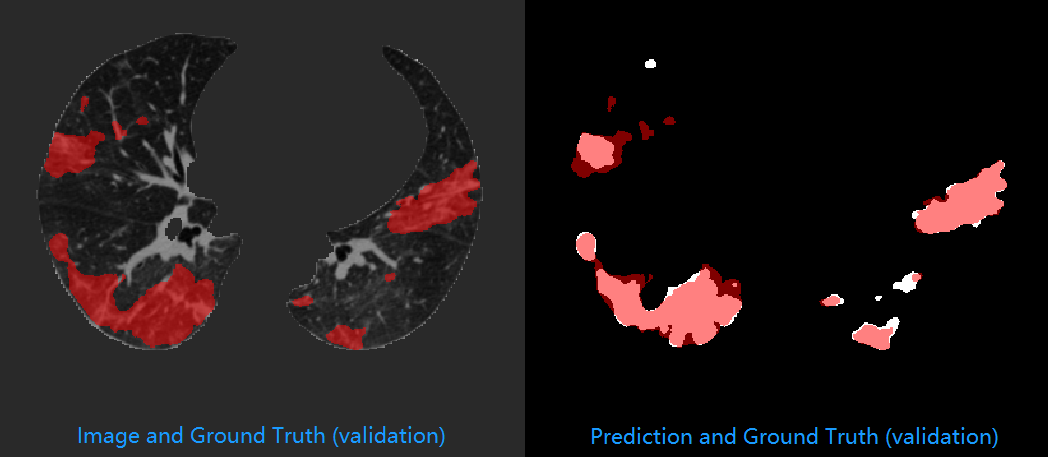
\includegraphics[width=0.8\textwidth]{img/experiment/Lung_result_val}
	\caption{Validation result of Lung infection segmentation; prediction shown in binary values}
	\label{fig:full_sup_lung_result}
\end{figure}

\begin{figure}[h]
	\centering
	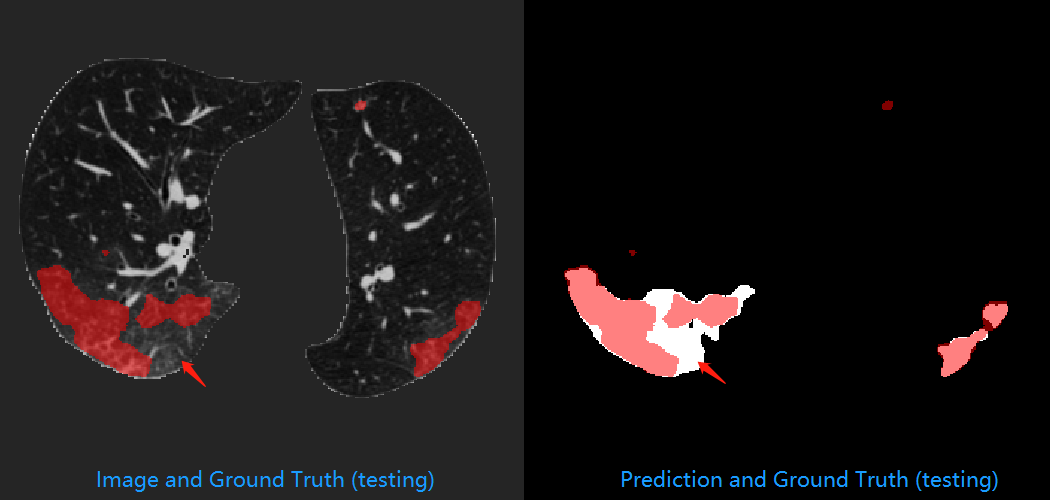
\includegraphics[width=0.8\textwidth]{img/experiment/Lung_result_test}
	\caption{Testing result of Lung infection segmentation; prediction shown in binary values. Note we argue that the label is a bit noisy}
	\label{fig:full_sup_lung_result}
\end{figure}


\newpage
\subsection{Training}
We compared the model trained from scratch and with transfer learning in this experiment. More specifically, we experimented two transfer learning initializations in this section. First we trained the Binary segmentation task with the images from NSCLC and MSD dataset, then the model was fine tuned using different methods suggested in work \cite{wang_improving_2019}: Freezing several layers in the Encoder and Fine tune the rest.

\subsubsection{Comparing training models}
We plot the validation curve using the small sample size trained on both plain UNet (left) and Attention-Gated UNet (right) in figure \ref{fig:unetvsatt}. We observed the UNet model with an attention gate intergration gives a more stable curve in validation.

\subsubsection{Training with very small sample size}
We first trained the model using a 10-40 split of training and validation, that is 10 volumes for training and 40 for validating. The intuition is to see how well the pre-trained network help when facing only a few training samples\\

\begin{figure}[h]
	\centering
	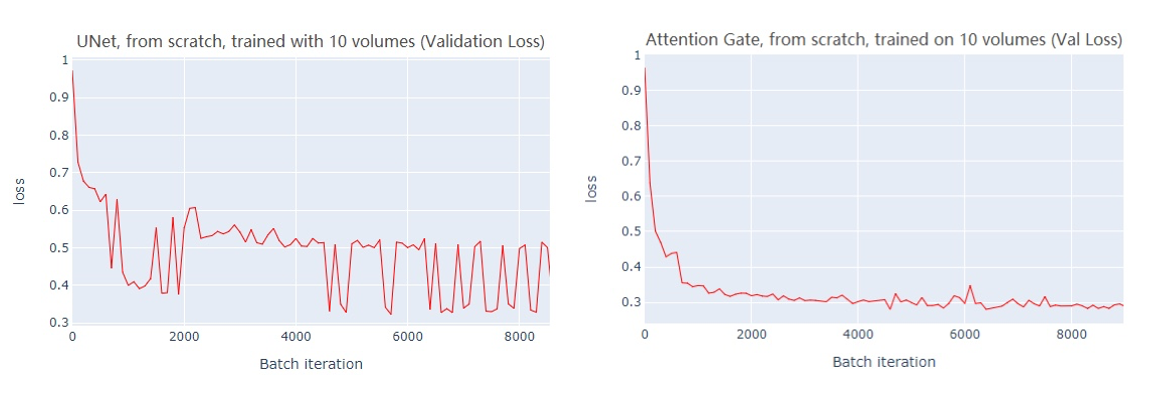
\includegraphics[width=\textwidth]{img/experiment/UnetvsAtt_fromscrath.png}
	\caption{Validation curve of training from scratch on UNet and Attention Gated UNet.}
	\label{fig:unetvsatt}
\end{figure}

%TODO change the freeze encoder part here
\begin{figure}
	\centering
	\includegraphics[width=\textwidth]{img/experiment/Unet_ft_10}
	\caption{Validation curve on one of the Cross Validation process. Model: Plain Unet; Fine tuned on 10 volumes.}
	\label{fig:fine_tune_unet}
\end{figure}

%TODO change the freeze encoder part here
\begin{figure}
	\centering
	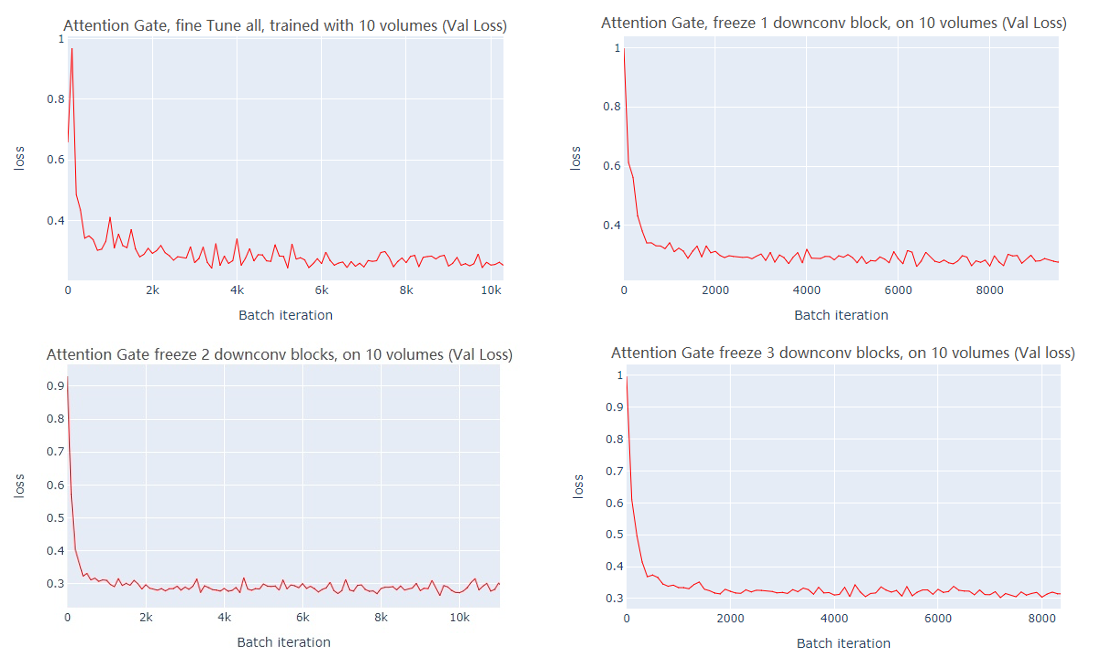
\includegraphics[width=\textwidth]{img/experiment/Att_ft_10}
	\caption{Validation curve on one of the Cross Validation process. Model: Plain Unet; Fine tuned on 10 volumes.}
	\label{fig:fine_tune_att}
\end{figure}


Figure \ref{fig:fine_tune_unet} (on UNet) and \ref{fig:fine_tune_att} (on Attention Gated UNet) plots the validation curve during fine-tuning using the model pretrained on non-covid Lung CT scans. First, the stability of Attention Gate still holds in the fine tuning process compared with the plain UNet. Second, compared with training from scratch, transfer learning yields better segmentation accuracy in test and validation on both of the models we experiments. The detailed Dice score is shown in table \ref{tab:10-transfer}. 

\begin{table}[h]
\centering
\begin{tabular}{l c c c c}
\hline
\hline
	&	Unet	&		&	Attention Gate	&		\\
	&	Validation	&	 Test	&	Validation	&	Test	\\
\hline
From Scratch		&	67.72	&	 63.49		& 71.97&	70.04	\\
Fine-Tune All	&	\textbf{71.74}	& 68.97	& \textbf{75.80}& 74.93		\\
Freeze 1 down conv	&	71.15	&	69.80	& 74.45&  74.02	\\
Freeze 2 down conv	&	69.87	&	69.02	& 73.53& 70.03	\\
Freeze 3 down conv	&	65.83	& 65.54 & 70.97&	70.10	\\
\hline
\end{tabular}
\caption{Validation and testing Dice score with two network architectures trained on the small sample (10 volumes) and validate on 40 volumes}
\label{tab:10-transfer}
\end{table}


\subsubsection{Larger training data}
We then trained our models with a relatively larger amount of data. In this experiment we did a 40-10 split, that is 40 for training and 10 for validation. Our results shows that, more data leads to a better performance even without transfer learning. Training from scratch with 40 volumes on average gives an accuracy of {\color{red} 76.82\% Dice score on the validation set while the best results in transfer learning with 10 volumes for training only reports 71.874\% trained with plain Unet. We have the same observation with the Attention Gate network.}\\


\textbf{Summarizing both the result in the two experiment above, we have the follow observations:}
\begin{enumerate}
	\item More training data gives better performance.
	\item We observed that, transfer learning offers a faster convergence compared to random initialization. Our explanation is that the pretrained model serve as a good starting point and some low-level features are already trained. This justification can be further explained by the SVCCA result we have in the next section.
	\item Fine tuning more layers gives a slightly better performance in our segmentation setup, that is more flexibility gives better accuracy. This observation follows the result in \cite{wang_improving_2019}.
	\item Altough transfer learning gives a better performance in both   of the experiments A and B, the accuracy gain is limited when facing a relatively larger amounts of training data.
	\end{enumerate}
\begin{table}[h]
	\centering
	\begin{tabular}{l c c c c}
\hline
\hline
				&	Unet		&			&	Attention Gate	&		\\
				&	Validation	&	 Test	&	Validation		&	Test	\\
\hline
From Scratch		&	76.84		&	76.32	&	78.42	&75.49	\\
Fine-Tune All	&	80.09		&	78.24	&	81.04	&80.45	\\
Freeze 1 down conv	&	80.01	&	78.18	&	80.75	&80.18	\\
Freeze 2 down conv	&	78.47	&	77.55	&	79.78	&73.24	\\
Freeze 3 down conv	&	73.52	&	72.85	&	75.63	&73.33	\\
\hline
\end{tabular}
\caption{Validation and testing Dice score with two network architectures trained on 40 volumes and validate on 10 volumes}
\end{table}
	


\subsection{SVCCA analysis on transfer learning}

\subsubsection{Network convergence during training}
We compared the convergence on each layer throughout the training process on the segmentation model. \cite{transfusion} reported that the network converged bottom up for a classification task during training. However, this is not exactly the case in our segmentation model.\\

\textbf{Network convergence with random initialization}\\

We first want to analyze the change of network layers from random initialization towards convergence using the SVCCA tool. We iterate through the dataloader and validate every 100 epochs and save the model if the result yield better performance.\\
\begin{figure}
	\centering
	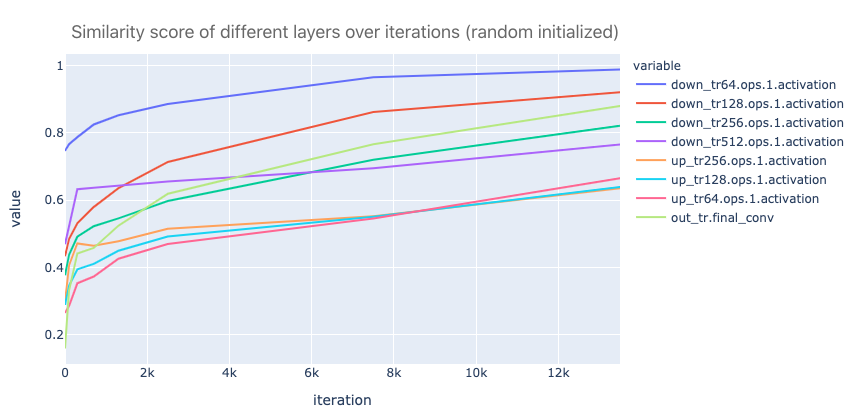
\includegraphics[width=0.8\textwidth]{img/SVCCA/CCA_score_scratch.png}
	\caption{CCA similarity score of each layer over training iterations (randomly initialized)}
	\label{fig:random_init_converge}
\end{figure}

Figure \ref{fig:random_init_converge} plots the similarity of latent space of each network layer using \textbf{random initialization}. 
\begin{itemize}
	\item We observed that, in general, encoder converged faster than decoder.
	\item The first down convolution block moved little from the initialized weights comparing the initialization to the converged model. Our explanation is that the first two convolutional layers mainly learn low level features such as edges and corners that are relatively easy.
	\item The similarity score in the output layer converged slightly faster than the other decoder part. Our explanation is that, the model performance (accuracy) increased faster in the first few number of iterations then slowly improved throughout the training.
	\item Although the similarity of the several Up-Convolution in the decoder part kept changing in the later stage of training, the output layer(out\_tr.finalconv in figure \ref{fig:random_init_converge}) did not moved much. One implication is that, Neural Network may learn different latent feature space while giving similar performance with respect to the accuracy. 
	\end{itemize}

\begin{figure}
	\centering
	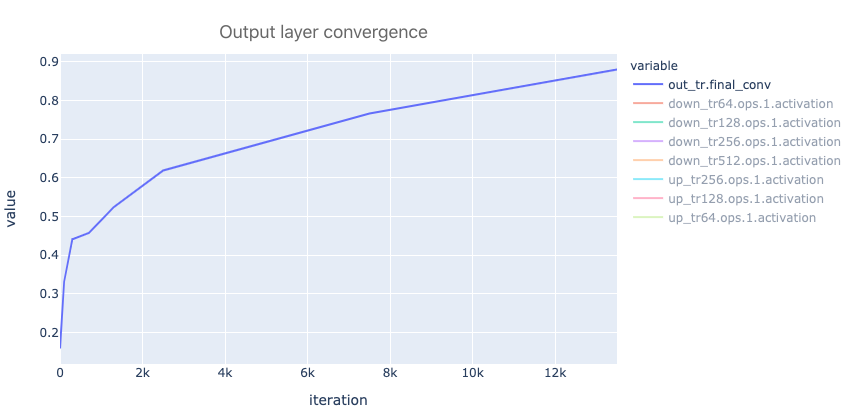
\includegraphics[width=0.8\textwidth]{img/SVCCA/from_scratch_output_layer.png}
	\caption{Filtering out the output layer convergence}
	\label{fig:random_init_converge}
\end{figure}

%\textbf{Train from scratch and transfer learning}\\
%We first compared the model before and after transfer learning. We saved the model that trained from scratch using the Covid dataset and the model pretrained using Lung dataset then fine-tuned to Covid dataset

\textbf{Network convergence during Fine-tuning}\\

Another question we asked is: \textbf{Is the convergence similar to random initialization when we have a pre-trained model?}
To test the convergence, we repeated the experiment in the previous section: Starting from a pre-trained model, we iterate through the Dataloader (containing 40 volumes sliced into 2D from the Axis view) and validate every 100 iterations. We saved the model of that epoch if the validation accuracy reported a better performance. Figure \ref{fig:transfer-convergence} plots the CCA similarity score of each saved model compared with the converged model.

\begin{figure}
	\centering
	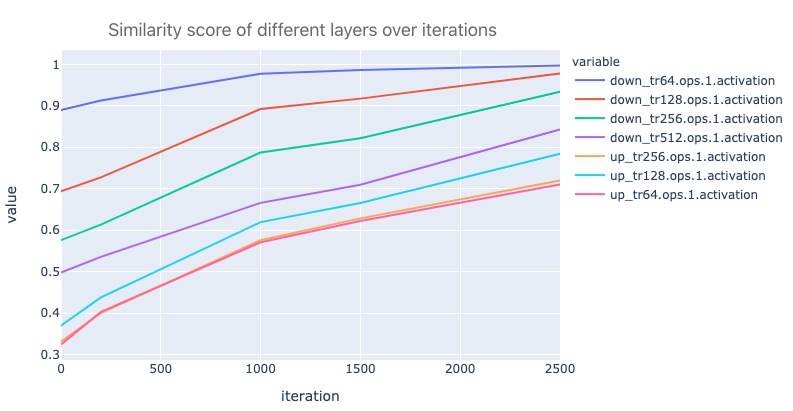
\includegraphics[width=0.8\textwidth]{img/SVCCA/CCA_score_transfer_learning}
	\caption{CCA similarity score of each layers over iterations during Fine-tuning}
	\label{fig:transfer-convergence}
\end{figure}

Comparing the similarity of feature map in the segmentation model, we observed the following behaviour when \textbf{Fine tuning} the network:
\begin{itemize}
	\item In the Encoder part, lower layers converged faster compared to higher layers. Specifically, down convolution reported higher similarity score from the beginning compared with the similarity score obtained when we trained from scratch, indicating the feature reuse in the encoder layers 
	\item \textbf{Feature resue} happened more in the lower layers for a good performance. In previous section, we performed some of the experiments with transfer learning through freezing different numbers of convolutional blocks. Fine tuning all layers or freezing the first few convolution blocks gives good accuracy in both small and larger training experients while freezing the whole encoder, however, degraded the performace by around 2 percent.\\
	
	 Analyzing the CCA similarity score in figure \ref{fig:transfer-convergence} gives a rough explanation to this observation that, comparing iteration 0 and the converged model, the first convolution block gives an similarity of 0.9 and the second down convolution block gives 0.7. The score decreased quickly when it comes to the rest of the layers. Note that bottleneck layer, namely down\_tr512 reported only 0.5 similarity comparing its initialization and converged result.
	\item Layers in the Decoder observed convergence almost at the same time, and the feature reuse is almost negligable since none of the similarity in the beginning is more than 0.5.
\end{itemize}

\subsubsection{Feature space comparison for transfer learning} 
%%TODO Change the title here
The last question we want to discuss in this section is: \textbf{How much did the model move given the amount of data it observed during the Fine-Tuning?}\\

Figure \ref{fig:transfer-convergence} shows that, although all layers output seen a higher similarity score as the iteration number increase, 
Down-Convolution layers in the Encoder moved much less compared to the rest of the model, yielding a slightly better feature reuse during Fine-Tuning, and the feature reuse decreased from lower layers to higher layers. The Decoder, however, gives a much lower similarity score (lower than 0.5) comparing the pre-trained initialization to the converged model. Figure \ref{fig:layer-wise-comparison} compared the layer-wise feature space similarity which showed the similar observation.

\begin{figure}
	\centering
	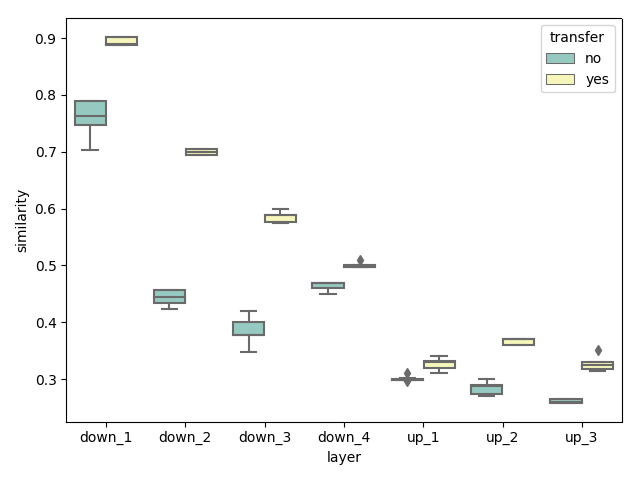
\includegraphics[width=0.8\textwidth]{img/SVCCA/sim_trans_withwithout.png}
	\caption{Layer-wise Comparison during training}
	\label{fig:layer-wise-comparison}
\end{figure}


\section{With unlabeled data}
We then consider leveraged unlablled data because in mid July, MosMed published unlabelled CT volumes. Thus, we continued our experiment to leveraged the unlabeled dataset. 
 We first fine tune a pre-trained model on the annotated dataset, take the encoder of the network. We cropped patches from the unannotated images, assign noisy label to them and train a mean-teacher style network using those cropped patches

\subsection{Experiment Setup}
Apart from the labelled dataset described in section 5.2, we downloaded 200 unlabeled volumes and first preprocessed the CT volumed as we described in chapter 3. Transfer learning in previous experiments gives a relatively faster convergence and better results, thus we followed the experiment in previous section using Fine-Tune-All method in this semi-supervise experiment.

\subsection{Training a coarse 3D segmentation}
The purpose of leveraging unlabelled data during training is to improve the generalization of the network so that it generalize better on unseen data. We want to crop more infection area to guide the segmentation model, so we first train a coarse 3D segmentation to generate a 'rough mask' of the image to guide the segmentation.
% TODO show an example here


\subsection{Psuedo Label Assignment -- Cosine Similarity in the feature space}
%TODO: change GAP to GMP
\begin{figure}[h]
	\centering
	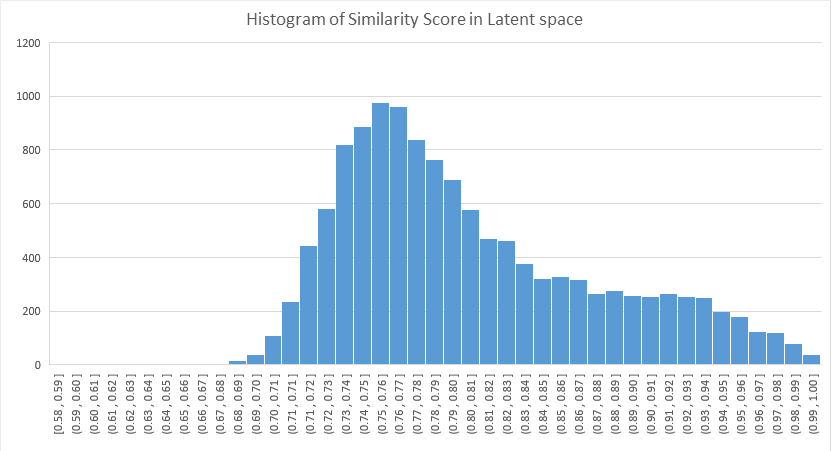
\includegraphics[width=0.8\textwidth]{img/semi-experiment/cosine_sim_histogram}
	\caption{Histogram of Cosine Similarity score}
	\label{fig:score_hist}
\end{figure}

Figure \ref{fig:score_hist} counts the occurence of similarity score over all sampled unlabeled patches. We took those samples with similarity score between 0.87 and 0.96 (sim $\in$ [0.87, 0.96]), and we assign the label of the annotated samples with highest similarity score. Figure \ref{fig:patches_noisy_mask} showed some examples of noisy labels assigned using this method.\\

We repeat this labeling process every epoch and iteratively select the labels based on the similarity score in the latent space. Table \ref{tab:num-epochs} reports the number of samples selected of each epoch during training.
\begin{table}[]
\centering
\begin{tabular}{l c}
\hline
\hline
Epoch & Samples selected \\
\hline
1     & 608              \\
2     & 570              \\
3     & 803              \\
4     & 710              \\
5     & 300              \\
6     & 480              \\
7     & 675              \\
8     & 752              \\
9     & 817              \\
10    & 841              \\
11    & 678              \\
12    & 357              \\
13    & 741              \\
14    & 512              \\
15    & 459              \\
16    & 784              \\
17    & 814    			\\
\hline         
\end{tabular}
\caption{Number of psuedo labeled samples selected each epoch}
\label{tab:num-epochs}
\end{table}
\begin{figure}[h]
	\centering
	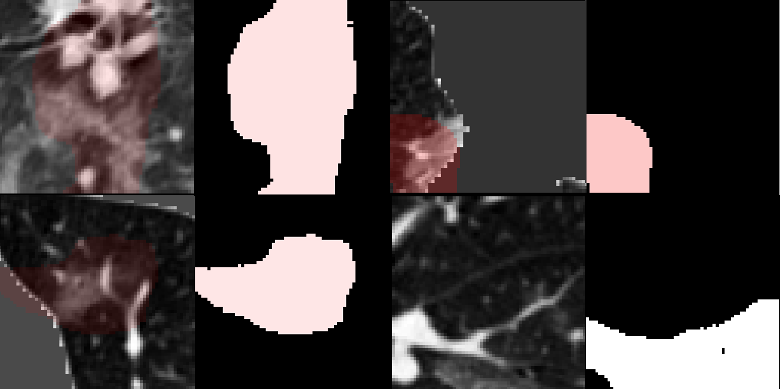
\includegraphics[width=0.8\textwidth]{img/semi-experiment/fake_assign_example}
	\caption{Example patches and noisy masks}
	\label{fig:patches_noisy_mask}
\end{figure}
\newpage
\subsection{Mean teacher training}
First we load the model save during the previous experiment in section 5.2. We prefer the model that give a relatively good starting point while not converged too much on the labelled training set. Thus, we load the model we saved after updated for 10 epochs and continued the training process. The validation and testing use the teacher model for better generalizability consideration. \\

\subsubsection{Updating Teacher models}
Note that here, the teacher model is not trained and updated using the observed samples but updated using the EMA updating process that each layer is an exponential moving average of the student model weights.\\

The student model however, is updated using a combination of consistency of predictions between the teacher model and the student model, as well as the segmentation accuracy using a combination of CE and Foreground Dice.

\subsubsection{Experiment results}
We trained the model with a smaller starting learning rate ($lr$ = 1e-4) when we continued our training from the loaded model. First both the teacher model and the student model observed a performance gain in the experiment. The teacher model in later training process reported
Figure \ref{fig:semi-1} \ref{fig:semi-2} and \ref{fig:semi-3} shows some examples on the testing set using the \textbf{Teacher Model} after the model convergence. Our semi-supervise setup observed a better segmentation accuracy.

\begin{table}[h]
\centering
\begin{tabular}{lll}
\hline
\hline
                                   & Validation & Testing \\
\hline
Best result in Supervised learning & 81.04      & 80.45   \\
Teacher model                      & 83.67      & 82.54   \\
Student model                      & 82.03      & 81.82  \\
\hline
\end{tabular}
\caption{Quantitative result using our model}
\label{tab:semi-table}
\end{table}


\begin{figure}
	\centering
	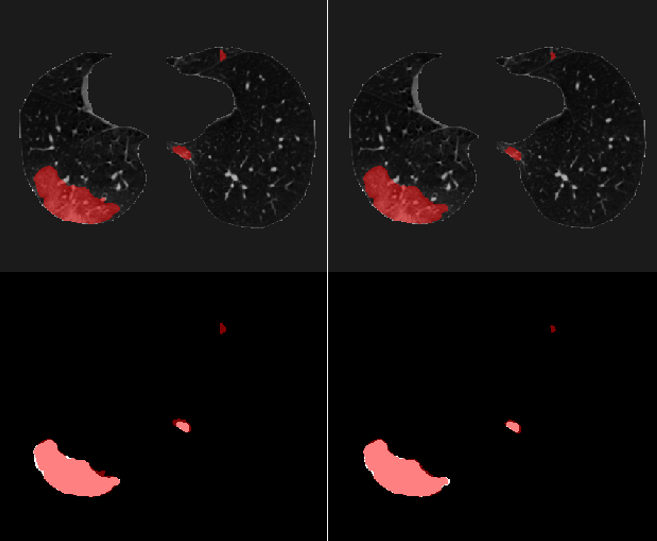
\includegraphics[width=0.7\textwidth]{img/experiment/semi_lung2}
	\caption{Example 1, when transferred attention gated UNet (Left) performance is as good as the accuracy with our semi-supervise setup (Right).}
	\label{fig:semi-1}
\end{figure}


\begin{figure}
	\centering
	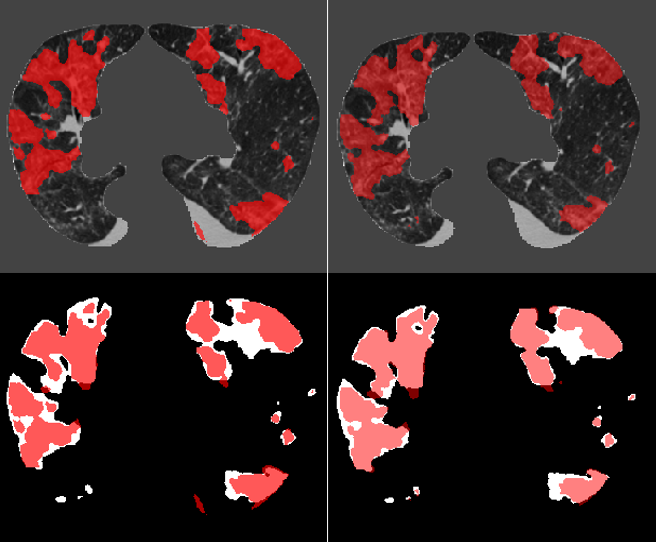
\includegraphics[width=0.7\textwidth]{img/experiment/semi_lung1}
	\caption{Example 2, observed a better prediction overlap using our semi-segmentation setup than the transferred attention gated UNet.}
	\label{fig:semi-2}
\end{figure}

\begin{figure}
	\centering
	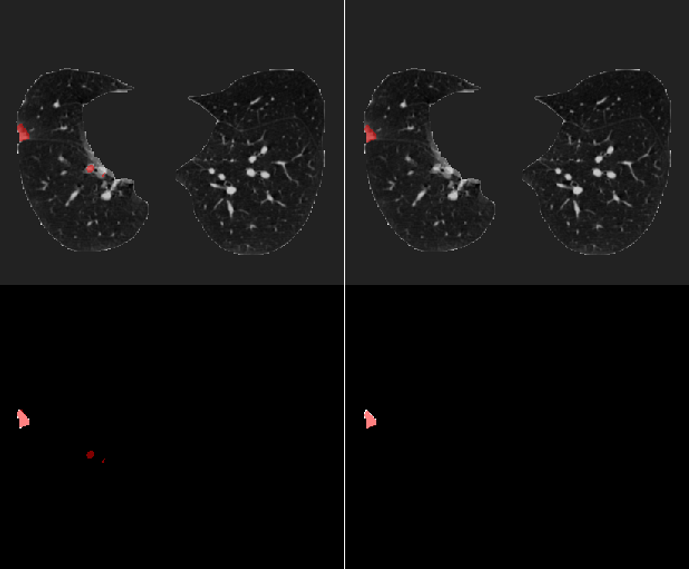
\includegraphics[width=0.7\textwidth]{img/experiment/semi_lung3}
	\caption{Example 3, observed a reduce in false positive area using our semi-segmentation setup.}
	\label{fig:semi-3}
\end{figure}


